\documentclass[a4paper,12pt]{article}

\usepackage[in]{fullpage}
\usepackage{tikz}
\usepackage[backend=bibtex,style=numeric-comp,sorting=none,sortcites=true]{biblatex}

\title{Qualifying Dissertation}
\author{James Baxter}
\date{}

\bibliography{literature} 

\begin{document}
\maketitle

\section{Introduction}
\begin{itemize}
  \item Popularity of Java
  \item Use of Java in embedded systems
  \item Importance of program correctness
  \item Importance of compiler correctness
  \item Difficulties of Java on embedded systems
  \item The need for a correct SCJ compiler for embedded systems
\end{itemize}

\section{Literature Review}

As the correctness of the compiler is of great importance to the correctness of the programs produced using it, there has been much research in the past into compiler correctness.
The approach that was used in the earliest works on compiler correctness, which is still widely used today, is to show that a diagram of the form shown in Figure~\ref{commuting-diagram} commutes.
\begin{figure}
  \begin{center}
    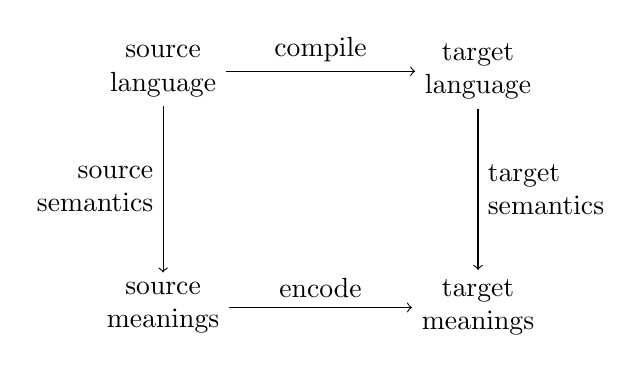
\begin{tikzpicture}
      \node[align=center] (S) at (0cm,3cm) {source\\language};
      \node[align=center] (T) at (4cm,3cm) {target\\language};
      \node[align=center] (M) at (0cm,0cm) {source\\meanings};
      \node[align=center] (U) at (4cm,0cm) {target\\meanings};
      
      \path (S) edge[->] node[align=center, above] {compile}           (T);
      \path (S) edge[->] node[align=right, left]   {source\\semantics} (M);
      \path (T) edge[->] node[align=left, right]   {target\\semantics} (U);
      \path (M) edge[->] node[align=center, above] {encode}            (U);
    \end{tikzpicture}
  \end{center}
  \caption{The commuting diagram used in the traditional approach to compiler verification}
  \label{commuting-diagram}
\end{figure}
Lockwood Morris\cite{morris1973} first observed that the commuting diagram approach was the usual approach to showing compiler correctness, though his version of the diagram had a decode function relating target meanings to source meanings.
Thatcher \emph{et al.}\cite{thatcher1979}, in extending Lockwood Morris' verification of a compiler, noticed that an encode function was more useful in reasoning and so included it in their diagram instead of the decode function. 
\end{document}